% !TEX program = xelatex
% =====================================================================
%  CS 6330 - Introduction to Data Science
%  Homework 4: Pairwise association (binary and continuous variables)
%  Author: Taek Lim
%
%  Build (from hw4/report/):  latexmk -C && latexmk -xelatex hw4_taeklim_report.tex
%
%  Every number comes from tables/numbers.tex (macros) and tables/p2_table.tex.
%  Rebuild them with: uv run python hw4/code/run_all.py
%  Figure paths are relative to this file: ../figures/*.png
% =====================================================================
\documentclass[11pt]{article}

\usepackage[letterpaper,margin=0.75in]{geometry}
\usepackage{fontspec}
\usepackage{amsmath}
\usepackage{booktabs}
\usepackage{graphicx}
\usepackage{float}        % [H]
\usepackage{caption}
\usepackage{xcolor}
\usepackage[hidelinks]{hyperref}
\usepackage{enumitem}

\captionsetup{font=small, labelfont=bf}
\setlength{\parindent}{0pt}
\setlength{\parskip}{0.5em}

\setlist{leftmargin=1.2em, itemsep=1pt, parsep=0pt, topsep=2pt}

% Generated table bodies end with a row break. LaTeX's \input hooks put tokens after the file,
% so \bottomrule would be misplaced; the primitive \@@input has no hook.
\makeatletter
\newcommand{\gentable}[1]{\@@input #1 }
\makeatother

% Generated by hw4/code/p3_report_tables.py. Do not edit.
\newcommand{\nCZz}{128}
\newcommand{\eCZz}{133.28}
\newcommand{\nCZo}{21}
\newcommand{\eCZo}{15.72}
\newcommand{\nCOz}{50}
\newcommand{\eCOz}{44.72}
\newcommand{\nCOo}{0}
\newcommand{\eCOo}{5.28}
\newcommand{\nRowZ}{149}
\newcommand{\nRowO}{50}
\newcommand{\nColZ}{178}
\newcommand{\nColO}{21}
\newcommand{\pOneN}{199}
\newcommand{\alphaLevel}{0.05}
\newcommand{\pOneHx}{0.8133}
\newcommand{\pOneHy}{0.4863}
\newcommand{\pOneMI}{0.0470}
\newcommand{\pOneMInats}{0.0326}
\newcommand{\pOneNMI}{0.0747}
\newcommand{\pOneMIp}{0.0018}
\newcommand{\pOnePerm}{10,000}
\newcommand{\pOneNullMax}{0.0525}
\newcommand{\pOneJac}{0.0000}
\newcommand{\pOneChi}{7.8784}
\newcommand{\pOneChiP}{0.0050}
\newcommand{\pOneYates}{6.4560}
\newcommand{\pOneYatesP}{0.0111}
\newcommand{\pOneMinE}{5.28}
\newcommand{\nA}{2{,}400}
\newcommand{\rA}{0.3809}
\newcommand{\tA}{20.17}
\newcommand{\dfA}{2{,}398}
\newcommand{\pA}{1.04\times 10^{-83}}
\newcommand{\rhoA}{0.3705}
\newcommand{\rabsA}{0.0176}
\newcommand{\rejA}{reject}
\newcommand{\nB}{110}
\newcommand{\rB}{0.9312}
\newcommand{\tB}{26.55}
\newcommand{\dfB}{108}
\newcommand{\pB}{3.74\times 10^{-49}}
\newcommand{\rhoB}{0.9275}
\newcommand{\rabsB}{0.0009}
\newcommand{\rejB}{reject}
\newcommand{\nC}{2{,}100}
\newcommand{\rC}{0.0412}
\newcommand{\tC}{1.89}
\newcommand{\dfC}{2{,}098}
\newcommand{\pC}{0.0592}
\newcommand{\rhoC}{0.0338}
\newcommand{\rabsC}{0.9911}
\newcommand{\rejC}{do not reject}
\newcommand{\bSharesC}{yes}


\begin{document}

\hfill Taek Lim \quad CS 6330 Homework 4: Pairwise Association

\bigskip
\textbf{Tooling.}
\begin{itemize}
  \item Tools: Python 3, NumPy, pandas, SciPy, matplotlib.
  \item Numbers: generated from saved result files, none typed by hand.
  \item Code: \texttt{hw4/code/} (\texttt{run\_all.py} runs every step). Code and write-up drafted with Claude Code.
  \item Significance level for every test: $\alpha = \alphaLevel$, fixed before the tests were run.
\end{itemize}

% =====================================================================
\section{Problem 1: Two binary genomic variants}

\textbf{Data.} \texttt{p1a.csv} holds \pOneN{} plants (rows) and two genomic variants (columns).
A 1 means the variant is present.
The file \texttt{p1b.csv} (199 $\times$ 15) also came with the data, but the assignment does not use it.

\subsection{Contingency table}

\begin{table}[H]
  \centering
  \caption{Observed counts of the two variants, with expected counts under independence in parentheses.
    Source: \texttt{hw4/results/p1\_contingency.csv}.}
  \label{tab:contingency}
  \begin{tabular}{lccc}
    \toprule
     & Variant 2 = 0 & Variant 2 = 1 & Row total \\
    \midrule
    Variant 1 = 0 & \nCZz{} (\eCZz) & \nCZo{} (\eCZo) & \nRowZ \\
    \midrule
    Variant 1 = 1 & \nCOz{} (\eCOz) & \nCOo{} (\eCOo) & \nRowO \\
    \midrule
    Column total  & \nColZ & \nColO & \pOneN \\
    \bottomrule
  \end{tabular}
\end{table}

Expected count: $E_{ij} = (\text{row}_i \times \text{col}_j) / n$.
The key cell is $n_{11} = \nCOo$: no plant carries both variants, while independence predicts \eCOo.

\subsection{Statistics}

Notation: $n_{11}$ = both present, $n_{10}$ = only variant 1, $n_{01}$ = only variant 2.

\begin{itemize}
  \item \textbf{Mutual information} (log base 2, so the unit is bits, lecture 15):
    $MI(X,Y) = H(X) + H(Y) - H(X,Y) = \sum_{x,y} p(x,y)\log_2 \frac{p(x,y)}{p(x)p(y)}$.
  \item \textbf{Jaccard index}: $J = n_{11} / (n_{11} + n_{10} + n_{01})$.
  \item \textbf{Chi-squared}: $\chi^2 = \sum_{i,j} (O_{ij} - E_{ij})^2 / E_{ij}$, with 1 degree of freedom.
\end{itemize}

\begin{table}[H]
  \centering
  \caption{Association statistics for \texttt{p1a.csv}.
    Source: \texttt{hw4/results/p1\_stats.csv}.}
  \label{tab:p1stats}
  \begin{tabular}{lll}
    \toprule
    Statistic & Value & Significance \\
    \midrule
    Entropy $H(\text{variant 1})$, $H(\text{variant 2})$ & \pOneHx{}, \pOneHy{} bits & \\
    \midrule
    \textbf{Mutual information} $MI$ & \textbf{\pOneMI{} bits} (\pOneMInats{} nats) & permutation $p = \pOneMIp$ \\
    \midrule
    Normalized MI, $MI/\sqrt{H(X)H(Y)}$ & \pOneNMI & \\
    \midrule
    \textbf{Jaccard index} $J$ & \textbf{\pOneJac} & \\
    \midrule
    \textbf{Chi-squared} $\chi^2$ (no continuity correction) & \textbf{\pOneChi} & $p = \pOneChiP$ \\
    \midrule
    Chi-squared with Yates correction & \pOneYates & $p = \pOneYatesP$ \\
    \bottomrule
  \end{tabular}
\end{table}

\textbf{MI significance.} I shuffled variant 2 \pOnePerm{} times and recomputed MI each time (lecture 15, slide 26).
The p-value is the share of shuffles with MI at least as large as the observed value.

\textbf{Findings.}
\begin{itemize}
  \item The two variants are associated. The chi-squared test rejects independence at $\alpha = \alphaLevel$ ($p = \pOneChiP$).
    The Yates-corrected test agrees ($p = \pOneYatesP$). So does the MI permutation test ($p = \pOneMIp$).
  \item The association is negative: the two variants never occur together.
    The table shows $\nCOo$ plants with both, against \eCOo{} expected.
  \item This explains the Jaccard index of \pOneJac. Jaccard counts only shared presence ($n_{11}$), so it is 0 here.
    Jaccard shows that the variants do not co-occur, but it cannot tell ``unrelated'' from ``mutually exclusive''.
  \item MI is small in absolute terms (\pOneMI{} bits, normalized \pOneNMI) because variant 2 is rare (\nColO{} of \pOneN{} plants).
    Knowing one variant removes little of the other's uncertainty.
    MI has no direction, so it does not show that the association is negative.
  \item The smallest expected count is \pOneMinE{} ($\geq 5$), so the chi-squared approximation is acceptable.
\end{itemize}

% =====================================================================
\section{Problem 2: Pairs of continuous gene expressions}

\textbf{Method.} For each file I computed the Pearson correlation $r$ between gene 1 and gene 2.
The null hypothesis is no association, $H_0: \rho = 0$.
The test statistic is $t = r\sqrt{n-2}/\sqrt{1-r^2}$ with $n-2$ degrees of freedom (lecture 14, slide 34).
The p-value is two-sided. I reject $H_0$ when $p < \alpha = \alphaLevel$.

\begin{table}[H]
  \centering
  \caption{Pearson correlation and p-value for each pair.
    Source: \texttt{hw4/results/p2\_stats.csv}.}
  \label{tab:p2}
  \begin{tabular}{llrrrll}
    \toprule
    Part & File & $n$ & $r$ & $t$ & $p$ & $H_0$ at $\alpha=\alphaLevel$ \\
    \midrule
    \gentable{tables/p2_table.tex}
    \bottomrule
  \end{tabular}
\end{table}

\subsection{Part (a): \texttt{p2a.csv}}

The Pearson correlation is $r_a = \rA$ with $p_a = \pA$ ($n = \nA$).
Because $p_a < \alphaLevel$, I \rejA{} the null hypothesis.
There is a statistically significant association between the two genes.
The direction is positive: when gene 1 is higher, gene 2 tends to be higher.
The magnitude is weak to moderate: the points form a wide cloud around an upward trend (Figure~\ref{fig:scatter}a).

\subsection{Part (b): \texttt{p2b.csv}}

The Pearson correlation is $r_b = \rB$ with $p_b = \pB$ ($n = \nB$).
Because $p_b < \alphaLevel$, I \rejB{} the null hypothesis.
There is a statistically significant association between the two genes.
The direction is positive, and the magnitude is very strong: the points lie close to a straight line (Figure~\ref{fig:scatter}b).

\subsection{Part (c): \texttt{p2c.csv}}

The Pearson correlation is $r_c = \rC$ with $p_c = \pC$ ($n = \nC$).
Because $p_c > \alphaLevel$, I \rejC{} the null hypothesis.
By the Pearson test, there is no statistically significant linear association.
The estimated linear association is close to zero, with a slightly positive sign.
However, the scatter plot shows a strong non-linear relationship (Figure~\ref{fig:scatter}c), discussed in part (e).

\subsection{Part (d): Scatter plots}

\begin{figure}[H]
  \centering
  \begin{minipage}{0.32\linewidth}\centering
    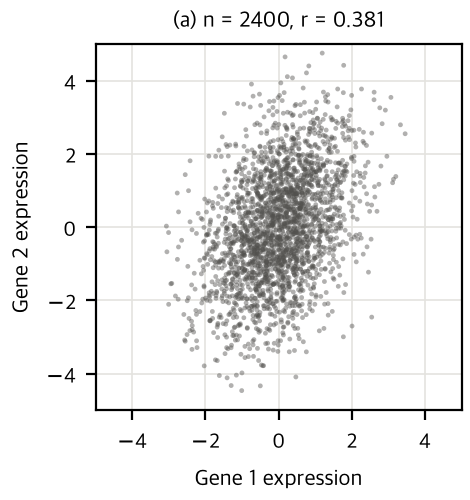
\includegraphics[width=\linewidth]{../figures/scatter_a.png}
  \end{minipage}\hfill
  \begin{minipage}{0.32\linewidth}\centering
    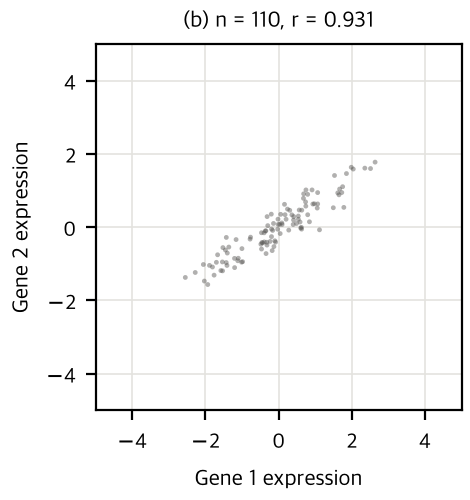
\includegraphics[width=\linewidth]{../figures/scatter_b.png}
  \end{minipage}\hfill
  \begin{minipage}{0.32\linewidth}\centering
    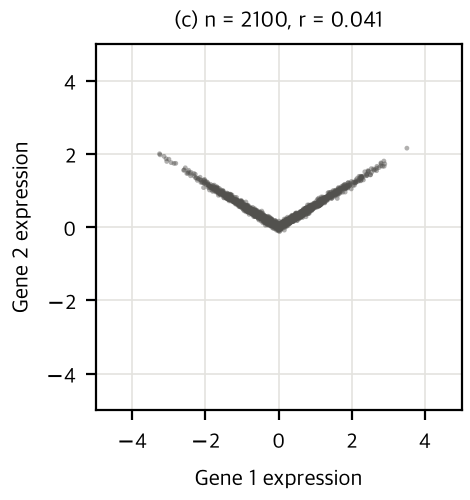
\includegraphics[width=\linewidth]{../figures/scatter_c.png}
  \end{minipage}
  \caption{Gene 1 (x) against gene 2 (y) for each file, on the same axis range. Panel titles give $n$ and Pearson $r$.
    Source: \texttt{hw4/figures/}.}
  \label{fig:scatter}
\end{figure}

\subsection{Part (e): Discussion}

\begin{table}[H]
  \centering
  \caption{Ranking of the three pairs, strongest association first.}
  \label{tab:rank}
  \begin{tabular}{lll}
    \toprule
    Criterion & Ranking & Basis \\
    \midrule
    Correlation $r$ & (b) $>$ (a) $>$ (c) & $\rB > \rA > \rC$ \\
    \midrule
    p-value (smaller = stronger evidence) & (a) $>$ (b) $>$ (c) & $\pA < \pB < \pC$ \\
    \midrule
    Scatter plots (my judgment) & (c) $>$ (b) $>$ (a) & shape and spread of the points \\
    \bottomrule
  \end{tabular}
\end{table}

\begin{enumerate}[label=\arabic*.]
  \item \textbf{By correlation:} (b), then (a), then (c).
    Pair (b) is almost perfectly linear ($r = \rB$). Pair (a) is weakly linear ($r = \rA$). Pair (c) has $r$ near zero ($\rC$).
  \item \textbf{By p-value:} (a), then (b), then (c).
    Pair (a) has the smallest p-value ($\pA$), even though its correlation is much weaker than that of (b).
    Pair (c) is not significant ($p = \pC$).
  \item \textbf{By the scatter plots:} (c), then (b), then (a).
    In (c) gene 2 is almost exactly a V-shaped function of gene 1, close to $|\text{gene 1}|$.
    Given gene 1, gene 2 is nearly fixed, so the dependence is the strongest of the three, but it is not linear.
    In (b) the points lie tightly along a straight line.
    In (a) the points form a broad tilted cloud.
  \item \textbf{Do they agree?} No. Each criterion picks a different strongest pair: (b) by $r$, (a) by $p$, and (c) by eye. Two reasons explain this:
    \begin{itemize}
      \item \textbf{The p-value depends on sample size, not only on strength.}
        It measures the evidence against $\rho = 0$, not the size of the association.
        Pair (a) has $n = \nA$ and pair (b) has $n = \nB$.
        With 2{,}400 samples, even a modest $r = \rA$ gives a large $t = \tA$.
        Pair (b) has a much larger $r$ but only 110 samples, so $t = \tB$ is only slightly larger.
        Because the degrees of freedom are much smaller for (b), its p-value ends up larger than that of (a).
        Both are far below $\alpha$. The difference between them reflects $n$, not strength.
      \item \textbf{Pearson's $r$ measures only linear association.}
        In (c) the left half of the points slopes down and the right half slopes up.
        The two halves cancel, so $r \approx 0$ and the test does not reject $H_0$.
        The genes are still strongly dependent: the correlation of $|\text{gene 1}|$ with gene 2 is $\rabsC$.
        Spearman's rank correlation ($\rhoC$) also misses it, because the relation is not monotonic.
        A measure that handles non-linear dependence, such as mutual information or MIC (lecture 15), would rank (c) high.
    \end{itemize}
    So a large $r$ shows a strong linear relation, and a small $p$ shows that an effect is unlikely to be zero.
    Neither replaces looking at the data.
\end{enumerate}

\textbf{Side note.} The gene 1 values of \texttt{p2b.csv} equal the first 110 gene 1 values of \texttt{p2c.csv} (checked: \bSharesC).
The two files share one variable but differ in gene 2 and in the shape of the relation.

\end{document}
